% !TEX TS-program = pdflatex
% !TEX encoding = UTF-8 Unicode

% This is a simple template for a LaTeX document using the "article" class.
% See "book", "report", "letter" for other types of document.

\documentclass[11pt]{article} % use larger type; default would be 10pt

\usepackage[utf8]{inputenc} % set input encoding (not needed with XeLaTeX)

%%% Examples of Article customizations
% These packages are optional, depending whether you want the features they provide.
% See the LaTeX Companion or other references for full information.

%%% PAGE DIMENSIONS
\usepackage{geometry} % to change the page dimensions
\geometry{letterpaper} % or letterpaper (US) or a5paper or....
% \geometry{margin=2in} % for example, change the margins to 2 inches all round
% \geometry{landscape} % set up the page for landscape
%   read geometry.pdf for detailed page layout information

\usepackage{graphicx} % support the \includegraphics command and options

% \usepackage[parfill]{parskip} % Activate to begin paragraphs with an empty line rather than an indent

%%% PACKAGES
\usepackage{booktabs} % for much better looking tables
\usepackage{array} % for better arrays (eg matrices) in maths
\usepackage{paralist} % very flexible & customisable lists (eg. enumerate/itemize, etc.)
\usepackage{verbatim} % adds environment for commenting out blocks of text & for better verbatim
\usepackage{subfig} % make it possible to include more than one captioned figure/table in a single float
% These packages are all incorporated in the memoir class to one degree or another...
\usepackage{indentfirst}
\usepackage{hyperref}
\usepackage{color}
\usepackage{float}

\hypersetup{
    bookmarks=true,         % show bookmarks bar?
    unicode=false,          % non-Latin characters in Acrobat’s bookmarks
    pdftoolbar=true,        % show Acrobat’s toolbar?
    pdfmenubar=true,        % show Acrobat’s menu?
    pdffitwindow=false,     % window fit to page when opened
    pdfstartview={FitH},    % fits the width of the page to the window
    pdftitle={My title},    % title
    pdfauthor={Author},     % author
    pdfsubject={Subject},   % subject of the document
    pdfcreator={Creator},   % creator of the document
    pdfproducer={Producer}, % producer of the document
    pdfkeywords={keyword1} {key2} {key3}, % list of keywords
    pdfnewwindow=true,      % links in new window
    colorlinks=true,       % false: boxed links; true: colored links
    linkcolor=blue,          % color of internal links (change box color with linkbordercolor)
    citecolor=green,        % color of links to bibliography
    filecolor=magenta,      % color of file links
    urlcolor=blue           % color of external links
}



\raggedright
\parindent=1.5em
\title{Jumping around hoops to find full period multipliers for a large prime modulus}
\author{Patrick Barringer and Michael Mason}

\begin{document}
\maketitle

\section{Introduction}
We were tasked with developing a Lehmer Random Number Generator for both 32 bit and 64 bit systems. The 32 bit is well explored in the textbook but the 64 bit case is only briefly mentioned, conveying no usable technical details. Upon realizing that no one had managed to find a good full period multiplier (FPM), $a$, and prime modulus, $m$, that takes full advantage of 64 bit arithmetic we endeavored to find one. The obvious choice for $m$ was $2^{63}-25$ as this is the largest prime that may be represented in a signed 64 bit integer. Now we merely had to find one full period multiplier- there was even a recipe in the book-and use that to find a multiplier that had good statistical properties and we would have accomplished our goals.
\\
The recipe in the book for finding a FPM involved simply going through every number and verifying that it cycled after m-1 calls. This approach was impractical for $2^{64}-25$ as this number is on the order of $10^{18}$ which would take approximately 15 years to verify a single FPM on the hardware available. This was an unacceptable amount of time as the project was due in a few short weeks, so another solution had to be devised. We had recently learned of the jump multiplier, a fairly simple way to jump some arbitrary number of calls ahead in a LRNG and thought that we may be able to verify FPMs by applying this concept. The basic idea was: if we were to jump ahead by a number larger then 1, say $10^9$ we could cycle through the entirety of the list much more quickly.
\section{Solution Overview}
The algorithm we devised involves selecting some $j$ that alows us to traverse the full cycle of numbers quickly (the choice of $j$ is discussed in detail in section \ref{choosej}). We then make $j$ calls to the random number generator storing the results in some collection with fast lookup. The third step is to use $a^j$ as our multiplier and make $\frac{m}{j}$ calls to the pRNG making sure that we do not generate a number that is also in the collection generated in the previous step. A graphical representation of this can be found in figure \ref{fig:fpmWithJump}.
\\
\begin{figure}[H]
\centering
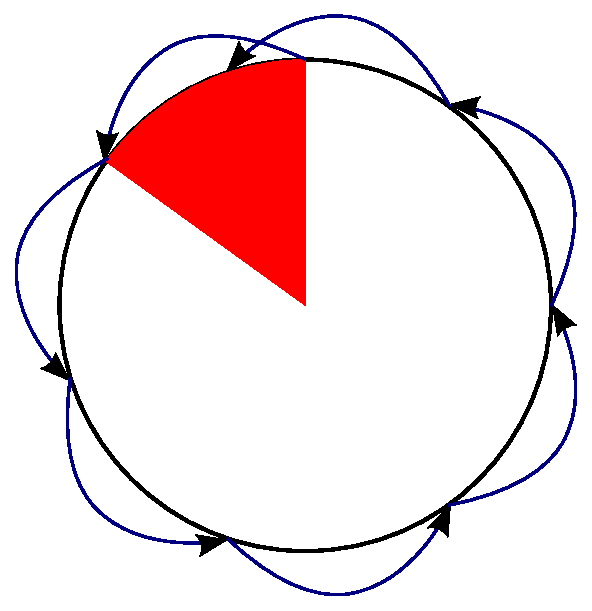
\includegraphics[width=0.34\textwidth]{fpmWithJump.pdf}
\caption{\label{fig:fpmWithJump} Demonstration of a full period multiplier.}
\end{figure}
In figure \ref{fig:fpmWithJump} the circle is the closed set of random numbers (the seed is at the 12o'clock position). The red slice is the component that we pull from the RNG using $a$ (the multiplier we are testing) as the multiplier, the blue arrows show the draws made using the $a^j \textrm{ mod } m$ multiplier. If the $a$ in question is a full period multiplier the number of jumps required to return to the red area will be $\frac{m}{j}$ if we return to the red area before $\frac{m}{j}$ pulls we know that $a$ is not full period. In this figure the jump size is exaggerated for clarity.

\section{Choosing $j$}\label{choosej}
To determine the optimal starting point of this algorithm we looked to try and minimize the number of pulls from the random number generator. The number of pulls from the random number generator $\nu(j)$ in terms of the jump size $j$ and the prime modulus $m$  is: 
\begin{equation}\label{numJumps}
\nu(j) = j + \frac{m}{j}
\end{equation}
minimizing equation \ref{numJumps} via a derivative
$$\nu'(j) = 1-\frac{m}{j^2}=0$$
\begin{equation}
\label{minJumps}
j=\sqrt{m}
\end{equation}
Using this as our jump distance we will need to make $2\sqrt{m}$ draws from the pRNG. Unfortunately we have no guarantees that $a^j \textrm{ mod } m$ is modulus compatible. If it is not we simply decrement $j$ until we find a $j$ that results in a  modulus compatible multiplier. Decrementing is preferable to incrementation because the algorithm requires we keep $j$ numbers in memory at a time.
\subsection{Problems encountered}
The major problem that we encountered using this methodology is that the calculation of $a^j \textrm{ mod } m$ is not a computation that can be solved traditionally when $j$ is on the order of $\sqrt{2^{63}-25}\approx2^{32}$ fortunately this is a common problem in cryptography and can be preformed in $O(\log_2(j))$ time. Unfortunately finding a modulus compatible $a$ with an modulus compatible $a^j \textrm{ mod } m$ is non-trivial and requires extensive trial and error. This is the primary computational difficulty. The other major problem with picking $j$ as the jump multiplier is the storage required for the ordered collection (approximately .25 Terabytes). We need this collection to have very fast lookup so we can not afford paging to disk. To this end  we chose 400 million as our $j$ due to the physical limitation of memory space.
% Commands to include a figure:

\end{document}
